% ===========================================
% Template for ICMC 2021 in Santiago, Chile (version1)
% adapted from earlier LaTeX paper templates for the ICMC, SMC, etc...
% by Rodrigo F. Cádiz rcadiz@uc.cl
% ===========================================

\documentclass{article}
\usepackage{icmc2021template}
\usepackage{times}
\usepackage{ifpdf}
\usepackage{soul}
\usepackage[english]{babel}
%\usepackage{cite}


%%%%%%%%%%%%%%%%%%%%%%%% Some useful packages %%%%%%%%%%%%%%%%%%%%%%%%%%%%%%%
%%%%%%%%%%%%%%%%%%%%%%%% See related documentation %%%%%%%%%%%%%%%%%%%%%%%%%%
%\usepackage{amsmath} % popular packages from Am. Math. Soc. Please use the 
%\usepackage{amssymb} % related math environments (split, subequation, cases,
%\usepackage{amsfonts}% multline, etc.)
%\usepackage{bm}      % Bold Math package, defines the command \bf{}
%\usepackage{paralist}% extended list environments
%%subfig.sty is the modern replacement for subfigure.sty. However, subfig.sty 
%%requires and automatically loads caption.sty which overrides class handling 
%%of captions. To prevent this problem, preload caption.sty with caption=false 
%\usepackage[caption=false]{caption}
%\usepackage[font=footnotesize]{subfig}

% ====================================================
% ================ Define title and author names here ===============
% ====================================================
%user defined variables
\def\papertitle{MusAssist: A Domain Specific Language for Music Notation}
\def\firstauthor{Ilana Shapiro}
\def\secondauthor{Second Author}
\def\thirdauthor{Third Author}
\def\fourthauthor{Fourth Author}
\def\fifthauthor{Fifth Author}
\def\sixthauthor{Sixth Author}

% adds the automatic
% Saves a lot of output space in PDF... after conversion with the distiller
% Delete if you cannot get PS fonts working on your system.

% pdf-tex settings: detect automatically if run by latex or pdflatex
\newif\ifpdf
\ifx\pdfoutput\relax
\else
   \ifcase\pdfoutput
      \pdffalse
   \else
      \pdftrue
  \fi
\fi

\ifpdf % compiling with pdflatex
  \usepackage[pdftex,
    pdftitle={\papertitle},
    pdfauthor={\firstauthor, \secondauthor, \thirdauthor},
    bookmarksnumbered, % use section numbers with bookmarks
    pdfstartview=XYZ % start with zoom=100% instead of full screen; 
                     % especially useful if working with a big screen :-)
   ]{hyperref}
  %\pdfcompresslevel=9

  \usepackage[pdftex]{graphicx}
  % declare the path(s) where your graphic files are and their extensions so 
  %you won't have to specify these with every instance of \includegraphics
  \graphicspath{{./figures/}}
  \DeclareGraphicsExtensions{.pdf,.jpeg,.png}

  \usepackage[figure,table]{hypcap}

\else % compiling with latex
  \usepackage[dvips,
    bookmarksnumbered, % use section numbers with bookmarks
    pdfstartview=XYZ % start with zoom=100% instead of full screen
  ]{hyperref}  % hyperrefs are active in the pdf file after conversion

  \usepackage[dvips]{epsfig,graphicx}
  % declare the path(s) where your graphic files are and their extensions so 
  %you won't have to specify these with every instance of \includegraphics
  \graphicspath{{./figures/}}
  \DeclareGraphicsExtensions{.eps}

  \usepackage[figure,table]{hypcap}
\fi

%setup the hyperref package - make the links black without a surrounding frame
\hypersetup{
    colorlinks,%
    citecolor=black,%
    filecolor=black,%
    linkcolor=black,%
    urlcolor=black
}


% ====================================================
% ================ Title and author info starts here ===============
% ====================================================
% Title.
% ------
\title{\papertitle}

% Authors
% Please note that submissions are anonymous, therefore 
% authors' names should not be VISIBLE in your paper submission.
% They should only be included in the camera-ready version of accepted papers.
% uncomment and use the appropriate section (1, 2 or 3 authors)
%
% Single address
% To use with only one author or several with the same address
% ---------------
%\oneauthor
%   {\firstauthor} {Affiliation \\ %
%     {\tt \href{mailto:author@uc.cl}{author@uc.cl}}}

%Two addresses
% the default spacing is 1.5in, but this can be reduced to 0.5in or less, if needed
%--------------
% \twoauthors
%   {1.5in}
%   {\firstauthor} {Affiliation1 \\  %
%     {\tt \href{mailto:author1@uc.cl}{author1@uc.cl}}}
%   {\secondauthor} {Affiliation2 \\  %
%     {\tt \href{mailto:author2@uc.cl}{author2@uc.cl}}}

% Three addresses
% the default spacing is 0.5in, but this can be reduced to 0.3in or less, if needed
% --------------
 \oneauthor
  %  {0.5in}
   {\firstauthor} {Pomona College \\ %
     {\tt \href{mailto:issa2018@mymail.pomona.edu}{issa2018@mymail.pomona.edu}}}
  %  {\secondauthor} {Affiliation2 \\ %
  %    {\tt \href{mailto:author2@myorg.org}{author2@myorg.org}}}
  %  {\thirdauthor} { Affiliation3 \\ %
  %    {\tt \href{mailto:author3@myorg.org}{author3@myorg.org}}}

% Four addresses
% the default spacing is 1.5in, but this can be reduced to 0.5in or less, if needed
% --------------
% \fourauthors
%   {1.5in}
%   {\firstauthor} {Affiliation1 \\ %
%     {\tt \href{mailto:author1@uc.cl}{author1@uc.cl}}}
%   {\secondauthor} {Affiliation2 \\ %
%     {\tt \href{mailto:author2@uc.cl}{author2@uc.cl}}}
%   {\thirdauthor} { Affiliation3 \\ %
%     {\tt \href{mailto:author3@uc.cl}{author3@uc.cl}}}
%   {\fourthauthor} { Affiliation4 \\ %
%     {\tt \href{mailto:author4@uc.cl}{author4@uc.cl}}}

% Five addresses
% the default spacing is 0.5in, but this can be reduced to 0.3in or less, if needed
% --------------
% \fiveauthors
%   {0.5in}
%   {\firstauthor} {Affiliation1 \\ %
%     {\tt \href{mailto:author1@uc.cl}{author1@uc.cl}}}
%   {\secondauthor} {Affiliation2 \\ %
%     {\tt \href{mailto:author2@uc.cl}{author2@uc.cl}}}
%   {\thirdauthor} { Affiliation3 \\ %
%     {\tt \href{mailto:author3@uc.cl}{author3@uc.cl}}}
%   {\fourthauthor} { Affiliation4 \\ %
%     {\tt \href{mailto:author4@uc.cl}{author4@uc.cl}}}
%   {\fifthauthor} { Affiliation5 \\ %
%     {\tt \href{mailto:author5@uc.cl}{author5@uc.cl}}}

% Six addresses
% the default spacing is 0.5in, but this can be reduced to 0.3in or less, if needed
% --------------
% \sixauthors
%   {0.5in}
%   {\firstauthor} {Affiliation1 \\ %
%     {\tt \href{mailto:author1@uc.cl}{author1@uc.cl}}}
%   {\secondauthor} {Affiliation2 \\ %
%     {\tt \href{mailto:author2@uc.cl}{author2@uc.cl}}}
%   {\thirdauthor} { Affiliation3 \\ %
%     {\tt \href{mailto:author3@uc.cl}{author3@uc.cl}}}
%   {\fourthauthor} { Affiliation4 \\ %
%     {\tt \href{mailto:author4@uc.cl}{author4@uc.cl}}}
%   {\fifthauthor} { Affiliation5 \\ %
%     {\tt \href{mailto:author5@uc.cl}{author5@uc.cl}}}
%   {\sixthauthor} { Affiliation6 \\ %
%     {\tt \href{mailto:author6@uc.cl}{author6@uc.cl}}}


% ====================================================
% =============== The document content starts here ===============
% ====================================================
\begin{document}
%
\capstartfalse
\maketitle
\capstarttrue
%
\begin{abstract}
MusAssist is an external DSL devised as a compositional aid for music notation. 
Users can change key signatures, start a new measure, and describe musical structures 
such as notes, rests, and custom chords in MusAssist’s straightforward syntax much in 
the same way they would when composing. MusAssist is unique in that users can also describe 
complex musical templates for triads and seventh chords, cadences, and the four primary 
harmonic sequences with desired length. The level of abstraction of a MusAssist template 
MusAssist matches that of the theoretical musical structure it describes (e.g. users can describe
 a harmonic sequence without lowering the abstraction level to chords and notes). This allows 
 users to write out specifications precisely at the conceptual levels of the musical structures 
 they would organically conceive when composing by hand. The musical expressions described by 
 the specifications are expanded out (i.e. the level of abstraction is fully lowered) by the 
 Haskell-based MusAssist compiler and are translated to MusicXML, a language accepted by most 
 major notation software, allowing for further manual editing. 
\end{abstract}
%

\section{Introduction}\label{sec:introduction}
MusAssist is an external domain specific language devised as a compositional aid for music
notation. It organically models a composer’s flow of thought by framing its syntax around the musical expressions
a composer conceives when writing. Users describe musical structures in MusAssist’s simple and
straightforward syntax just as they would when composing. In other words, users
describe a composition in MusAssist, and MusAssist writes out the music via these instructions.
Fundamentally, MusAssist supports notes (including rests) and custom chords (i.e. any desired collection of notes)
in the octave and key of choice, as well as change the key signature or start a new measure at any
point. MusAssist is unique in that users can also describe complex musical templates;
specifically, templates for chords (all types of triads and seventh chords in any inversion), cadences
(perfect authentic, imperfect authentic, plagal, half, deceptive), and harmonic sequences (ascending
fifths, descending fifths, ascending 5-6, descending 5-6) of a desired length. The level of abstraction of a 
template in MusAssist matches that of the musical structure it describes (e.g. users can define a high-level harmonic 
sequence without needing to lower the level of abstraction to chords and notes). This allows users to write 
out a specification precisely at the conceptual level of the structure. The musical expression 
described by this specification will then be completely expanded out (i.e. the level of abstraction will be 
fully lowered) by the Haskell-based MusAssist compiler.

The target language of the MusAssist compiler is MusicXML, itself a DSL that is an extension of
XML (Extensible Markup Language). MusicXML is accepted by most major notation software programs (such as MuseScore). 
Thus, once a user has described a composition in MusAssist, they can open the resulting MusicXML file in MuseScore or another
program for further customization and editing, thus bypassing the need to write out complex musical templates by hand at a 
note- and chord-level of abstraction. Beyond a professional music compositional aid, MusAssist may be particularly 
helpful to music students as an educational tool, enabling them to visualize the relationship between a theortical musical structure 
and its expanded form, such as a cadence and the chords resulting from its expansion.

A MusAssist user need not have any computing background, though they should understand
music theory through chord and cadence types, as well as harmonic sequences.

This template includes all the information about formatting manuscripts for the ICMC 2021 Conference. When preparing your submission, please use either the MS-Office or LaTeX templates provided. Please follow these guidelines to give the final proceedings a uniform look. Authors will be {\em required} to make any necessary typographic corrections and changes before publication. If you have any questions, please contact the ICMC 2021 Organizers.

This template can be downloaded from the ICMC 2021 web site (\texttt{http://icmc2021.org/}).

\section{Page size and format}\label{sec:page_size}
The proceedings will be formatted as {\em portrait A4-size paper (21.0cm $\times$ 29.7cm)}. All material on each page should fit within a rectangle of 17.2cm $\times$ 25.2cm, centered on the page, beginning 2.0cm from the top of the page and ending with 2.5cm from the bottom. The left and right margins should be 1.9cm. The text should be in two 8.2cm columns with a 0.8cm gutter. All {\em text} must be in a two-column format, and justified.

\section{Typeset Text}\label{sec:typeset_text}

\subsection{Normal or Body Text}\label{subsec:body}
Please use a 10~pt (point) Times family font (i.e., Times New Roman). Sans-serif fonts or non-proportional fonts can be used only for special purposes, such as distinguishing source code text.

The first paragraph in each section should not be indented, but all other paragraphs should be. (Again, these have all been set in the styles provided.)

% this inserts a column-break
%\pagebreak

\subsection{Title and Authors}
The title is 16~pt Times, bold, upper case, centered. Authors' names are centered. The lead author's name is to be listed first (left-most), and the co-authors' names after. If the addresses for all authors are the same, include the address only once, centered. If the authors have different addresses, put the addresses, evenly spaced, under each authors' name.

\subsection{First Page Copyright Notice}
Please include the copyright notice exactly as it appears here in the lower left-hand corner of the page. It is set in 8~pt Times, one column in width, and should not descend into the  page margins (i.e. it should keep clear of the 1" margin at the bottom of the page).

\subsection{Page Numbering, Headers and Footers}
Do not include headers, footers or page numbers in your submission. These will be added when the publications are assembled.

\section{Headings}
First level headings are in Times 12pt bold, centered with 1 line of space above the section head, and 1/2 space below it.  For a section header immediately followed by a subsection header, the space should be merged.

\subsection{Second Level Headings}
Second level headings are in Times 10~pt bold, flush left,
with 1 line of space above the section head, and 1/2 space below it.
The first letter of each significant word is capitalized.

\subsubsection{Third and further Level Headings}
Third level headings are in Times 10~pt italic, flush left, with 1/2 line of space above the section head, and 1/2 space below it. The first letter of each significant word is capitalized.

Using more than three levels of headings is strongly discouraged.

\pagebreak

\section{Equations, Figures, Footnotes}

\subsection{Equations}
Equations should be placed on separated lines and numbered.
The number should be on the right side, in parentheses.
\begin{equation}
E=mc^{2}.
\label{eq:Emc2}
\end{equation}

\subsection{Figures, Tables and Captions}
All artwork must be centered, neat, clean, and legible. All lines should be very dark for purposes of reproduction and artwork should not be hand-drawn. The proceedings will be distributed in electronic form only, therefore color figures are allowed. However, you may want to check that your figures are understandable even if they are printed in black-and-white.
\begin{table}[h]
 \begin{center}
 \begin{tabular}{|l|l|}
  \hline
  String Value & Numeric value \\
  \hline
  Hello ICMC & 2021 \\
  \hline
 \end{tabular}
\end{center}
 \caption{Table captions should be placed below the table.}
 \label{tab:example}
\end{table}

Numbers and captions of figures and tables always appear below the figure/table. Leave 1 line space between the figure or table and the caption. Figure and tables are numbered consecutively. Captions should be Times 10~pt. Place tables/figures in text as close to the reference as possible, and preferably at the top of the page.

\begin{figure}[h]
\centering
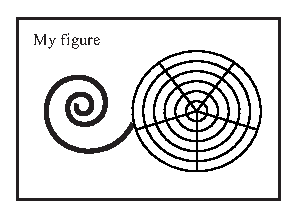
\includegraphics[width=0.9\columnwidth]{figure.eps}
\caption{Figure captions are placed below the figure, exactly like this.\label{fig:example}}
\end{figure}

Always refer to tables and figures in the main text, for example:
see Figure \ref{fig:example} and \tabref{tab:example}. 
Place Tables/Figures in text as close to the reference as possible.
Figures and tables may extend across both columns to a maximum width of 17.2cm.

Vectorial figures are preferred. 
When using {\texttt{Matlab}}, 
export using either Postscript or PDF format. 
Also, in order to optimize readability, the font size of text within a figure should be at list identical to footnote font size. If bitmap figures are used, please make sure that the resolution is enough for print quality. 

\subsection{Footnotes}
Indicate footnotes with a number in the text.\footnote{This is a footnote.}
Use 8~pt type for footnotes. Place the footnotes at the bottom of the page 
on which they appear. 
Precede the footnote with a 0.5~pt horizontal rule.

%\newpage

\section{Citations}
All bibliographical references should be listed at the end, inside a section named ``REFERENCES''.

References must be numbered {\ul {in order of appearance}}, {\em not} alphabetically. Please avoid listing references that do not appear in the text.

Reference numbers in the text should appear within square brackets, such as 
in~\cite{Someone:09} or~\cite{Someone:04,Someone:13}.

The reference format is the standard IEEE one. We recommend using BibTeX to create the reference list.


\section{Conclusions}
Please, submit full-length papers. Submission is fully electronic and automated through the Conference Management System. 
{\ul{Do not}} send papers directly by e-mail.

\begin{acknowledgments}
At the end of the Conclusions, acknowledgements to people, projects, funding agencies, etc. can be included after the second-level heading ``Acknowledgments'' (with no numbering).
\end{acknowledgments} 

%%%%%%%%%%%%%%%%%%%%%%%%%%%%%%%%%%%%%%%%%%%%%%%%%%%%%%%%%%%%%%%%%%%%%%%%%%%%%
%bibliography here
\bibliography{icmc2021template}

\end{document}
